\hfill\small{9 Jan 2024}
\vspace{0.5em}
\hrule
\vspace{-0.5em}
\section{Lecture 2 --- Phase Portraits}

Consider the system \(\dot{x} = f(x) \) which has an equillibrium point \(x^{\star} \in \mathbb{R}\)
Thus,
\[
    \left . \dot{x}  \right |_{x=x^{\star}} \iff f(x^{\star}) = 0
\]  
\begin{example}[Linear System]
    Consider the case of a linear system given by \(\dot{x} = ax\).
     Then, the equillibrium point is \(x^{\star} = 0\). The solution to the system
     is given by \(x(t) = e^{at} x_0\). The qualitative behaviour of the system 
     depending upon the value of \(a\) is given by the following ``1-D'' phase portrait diagram.

     \begin{center}
        \begin{tikzpicture}
            % Axis lines
            \draw[-] (-2,0) -- (2,0) node[below right] {$x$};
            
            % Arrows pointing towards each other
            \draw[<->] (1,0) -- (-1,0) node[midway]{};
            
            % Origin point
            \draw[] (0,-0.1) -- (0,0.1);
            \node[below right]{$0$};
            \node[right]at (3,0) {$a < 0$};
          \end{tikzpicture}

          \begin{tikzpicture}
            % Axis lines
            \draw[-] (-2,0) -- (2,0) node[below right] {$x$};
            
            % Arrows pointing towards each other
            \draw[>-<] (1,0) -- (-1,0) node[midway]{};
            
            % Origin point
            \draw[] (0,-0.1) -- (0,0.1);
            \node[below right]{$0$};
            \node[right]at (3,0) {$a > 0$};
          \end{tikzpicture}
    \end{center}
    Where the arrows shows the evolution of the trajectory of the system. At \(a = 0\), the
    the entire real line is the equillibria of the system.
\end{example}

\begin{example}[Nonlinear System]
    We will consider a bunch of non linear systems with varying qualitative behaviour.
    \begin{itemize}
        \item \(\dot{x} = x^{2} \quad x \in \mathbb{R} \)
        \begin{center}
            \begin{tikzpicture}
                % Axis lines
                \draw[-] (-2,0) -- (-1,0) node[] {};
                \draw[-] (1,0) -- (2,0) node[below right] {$x$};
                
                % Arrows pointing towards each other
                \draw[<-<] (1,0) -- (-1,0) node[midway]{};
                
                % Origin point
                \draw[] (0,-0.1) -- (0,0.1);
                \node[below right]{$0$};
              \end{tikzpicture}
        \end{center}
        \item \(\dot{x} = x^{2} - 1 \quad x \in \mathbb{R}\) 
        \begin{center}
            \begin{tikzpicture}
                % Axis lines
                \draw[-] (-3,0) -- (-2,0) node[] {};
                \draw[>-<] (-2,0) -- (0,0) node[] {};
                \draw[->] (0,0) -- (2,0) node[] {};
                \draw[-] (2,0) -- (3,0) node[below right] {$x$};
                
                
                \draw[] (-1,-0.1) -- (-1,0.1);
                \node [below right] at (-1,0) {$-1$};
                \draw[] (1,-0.1) -- (1,0.1);
                \node [below right] at (1,0) {$1$};
              \end{tikzpicture}
        \end{center}
        \item \(\dot{x} = 1\quad x \in \mathbb{R}\)
        \begin{center}
            \begin{tikzpicture}
                % Axis lines
                \draw[-] (0,0) -- (2,0) node[below right] {$x$};
                
                % Arrows pointing towards each other
                \draw[->] (-2,0) -- (0,0) node[midway]{};
              \end{tikzpicture}
        \end{center}
        \item \(\dot{x} = \sin (x) \quad x \in \mathbb{R}\)
        \begin{center}
            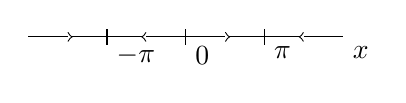
\begin{tikzpicture}
                % Axis lines
                \draw[-] (1.5,0) -- (2,0) node[below right] {$x$};
                % Arrows pointing towards each other
                \draw[>-<] (0.5,0) -- (1.5,0) node[midway]{};
                \draw[-] (-0.5,0) -- (0.5,0) node[midway]{};
                \draw[>-<] (-1.5,0) -- (-0.5,0) node[midway]{};
                \draw[-] (-2,0) -- (-1.5,0) node[midway]{};
                \draw[] (-1,-0.1) -- (-1,0.1);
                \draw[] (1,-0.1) -- (1,0.1);
                \draw[] (0,-0.1) -- (0,0.1);
                \node [below right] at (0,0) {$0$};
                \node [below right] at (1,0) {$\pi$};
                \node [below right] at (-1,0) {$-\pi$};
              \end{tikzpicture}
        \end{center}
    \end{itemize}
    
\end{example}

\subsection{2D Phase Portraits}
Let the two dimensional system be defined by
\[
    \dot{x}_1 = f_1(x_1, x_2) \quad \dot{x}_2 = f_2(x_1, x_2) \implies \dot{x} = f(x)  
\]
The phase portrait in some rough sense can be thought of as the ``trajectory'' of the system,
and where we care about the slope of the vector field of \(f(x)\) is given by:
\[
    \frac{\dot{x}_2}{\dot{x}_1} = \frac{f_2(x)}{f_1(x)}  
\] 
The phase portrait of the linear system can be easily understood via the jordan normal form
of the system.

Consider the system given by, \(\dot{x} = Ax \), and the linear transformation given by \(y = Px\),
Thus we get,
\[
    \dot{y} = P\dot{x} = PAx = PAP^{-1}y = Jy  
\]  
where \(J\) is the jordan normal form of \(A\).

We can have one of the 3 cases of the jordan form. The forms with their characteristic
polynomials are given by:

\[
    \begin{aligned}
        J_1 &= \begin{bmatrix}
            \lambda_1  &  0 \\
            0 &  \lambda _2 \\
        \end{bmatrix} \implies  p(s) = (s-\lambda _1) (s-\lambda _2)\\
        J_2 &= \begin{bmatrix}
            \lambda_1  &  1 \\
            0 &  \lambda _1 \\
        \end{bmatrix} \implies  p(s) = (s-\lambda _1) ^2\\
        J_3 &= \begin{bmatrix}
            \alpha  &  -\beta  \\
            \beta  &  \alpha  \\
        \end{bmatrix} \implies  p(s) = (s-\alpha) ^2 + \beta ^2\\
    \end{aligned}
\]
The solution of the equation in the transformed coordinates is given by:
\[
    y(t) = e^{Jt} y(0) \implies  x(t) = P ^{-1} e^{Jt} P x(0)
\]
Thus, the solution can be split into three cases similar to the one done above\\
\textbf{Case 1:}
\[
    y_1(t) = e^{\lambda _1 t} y_1(0) \quad y_2(t) = e^{\lambda _2 t} y_2(0)
\]
Thus, depending on the value of \(\lambda _1\) and \(\lambda _2\), we can have the following
phase portraits:\\
\medskip%
\begin{minipage}
    {0.5\textwidth}
    

\begin{tikzpicture}[
    declare function={f(\x,\y) = -3 * \x ;},
    declare function={g(\x,\y) = -1 * \y ;}
    ]
    \begin{axis}[
        simplePhase,
        title={$\lambda_1<\lambda _2<0$},
        width=\textwidth
      ]
      \addplot3 (x,y,0);
    \end{axis}
  \end{tikzpicture}

\end{minipage}
\begin{minipage}
    {0.5\textwidth}
    \begin{center}
    \begin{tikzpicture}[
        declare function={f(\x,\y) = 3 * \x ;},
        declare function={g(\x,\y) = 1 * \y ;}
        ]
        \begin{axis}[
            simplePhase,
            title={$\lambda_1<\lambda _2<0$},
            width=\textwidth
          ]
          \addplot3 (x,y,0);
        \end{axis}
      \end{tikzpicture}
\end{center}
\end{minipage}
\centerline{\begin{minipage}
    {0.5\textwidth}
    \begin{center}
    \begin{tikzpicture}[
        declare function={f(\x,\y) = 1 * \x ;},
        declare function={g(\x,\y) = 1 * \y ;}
        ]
        \begin{axis}[
            simplePhase,
            title={$\lambda_1<\lambda _2<0$},
            width=\linewidth
          ]
          \addplot3 (x,y,0);
        \end{axis}
      \end{tikzpicture}
    \end{center}
\end{minipage}}\\
% \begin{center}
    \begin{tikzpicture}[
        declare function={f(\x,\y) = 1 * \x ;},
        declare function={g(\x,\y) = 1 * \y ;}
        ]
        \begin{axis}[
            simplePhase,
            title={$\lambda_1<\lambda _2<0$},
            width=\linewidth
          ]
          \addplot3 (x,y,0);
        \end{axis}
      \end{tikzpicture}
    \end{center}

% 

\begin{tikzpicture}[
    declare function={f(\x,\y) = -3 * \x ;},
    declare function={g(\x,\y) = -1 * \y ;}
    ]
    \begin{axis}[
        simplePhase,
        title={$\lambda_1<\lambda _2<0$},
        width=\textwidth
      ]
      \addplot3 (x,y,0);
    \end{axis}
  \end{tikzpicture}

% \begin{center}
    \begin{tikzpicture}[
        declare function={f(\x,\y) = 3 * \x ;},
        declare function={g(\x,\y) = 1 * \y ;}
        ]
        \begin{axis}[
            simplePhase,
            title={$\lambda_1<\lambda _2<0$},
            width=\textwidth
          ]
          \addplot3 (x,y,0);
        \end{axis}
      \end{tikzpicture}
\end{center}
\medskip
\textbf{Case 2:}
\[
    \begin{aligned}
        y_1(t) &= e^{\lambda t} \left(   y_1(0) + t y_2(0)  \right)\\
        y_2(t) &= e^{\lambda t} y_2(0)
    \end{aligned}
\]
Simillary, we can have the following phase portraits depending on the value of \(\lambda\):\\
\medskip%
\begin{minipage}
    {0.5\textwidth}
    \begin{center}
    \begin{tikzpicture}[
        declare function={f(\x,\y) = -2 * \x + \y ;},
        declare function={g(\x,\y) = -2 * \y ;}
        ]
        \begin{axis}[
            simplePhase,
            title={$\lambda < 0$: Improper Stable Node},
            width=\textwidth
          ]
          \addplot3 (x,y,0);
          \addplot +[magenta] {0.5 * x};
        \end{axis}
      \end{tikzpicture}
    \end{center}
    
\end{minipage}
\begin{minipage}
    {0.5\textwidth}
    \begin{center}
    \begin{tikzpicture}[
        declare function={f(\x,\y) = 2 * \x + \y ;},
        declare function={g(\x,\y) = 2 * \y ;}
        ]
        \begin{axis}[
            simplePhase,
            title={$\lambda > 0$: Improper Unstable Node},
            width=\textwidth
          ]
          \addplot3 (x,y,0);
          \addplot +[magenta] {-0.5 * x};
        \end{axis}
      \end{tikzpicture}
    \end{center}
    
\end{minipage}\\
\medskip%
\textbf{Case 3:} Let \( r\coloneqq \sqrt{y_1 ^{2} + y_{2^{2} }  } \) and \(\theta \coloneqq \tan ^{-1}  \left( \frac{y_2}{y_1}  \right) \)
Substituing the values of \(y_1\) and \(y_2\) in the equation, and simplifying, we get:
\[
    \dot{r} = \alpha r \quad \dot{\theta} = \beta 
\]
Thus, switching in the polar form, the transformed system are evolving independently of each other.
The phase portrait is given by:\\
\medskip%
\begin{minipage}
    {0.5\textwidth}
    \begin{center}
    \begin{tikzpicture}[
        declare function={f(\x,\y) = -2 * \x - \y ;},
        declare function={g(\x,\y) = \x - 2 * \y ;}
        ]
        \begin{axis}[
            simplePhase,
            title={$\lambda > 0$: Stable Focus},
            width=\textwidth
          ]
          \addplot3 (x,y,0);
        \end{axis}
      \end{tikzpicture}
    \end{center}
    
\end{minipage}
\begin{minipage}
    {0.5\textwidth}
    \begin{center}
    \begin{tikzpicture}[
        declare function={f(\x,\y) = 2 * \x - \y ;},
        declare function={g(\x,\y) = \x + 2 * \y ;}
        ]
        \begin{axis}[
            simplePhase,
            title={$\lambda < 0$: Unstable Focus},
            width=\textwidth
          ]
          \addplot3 (x,y,0);
        \end{axis}
      \end{tikzpicture}
    \end{center}
    
\end{minipage}\\
% 

\begin{tikzpicture}[
    declare function={f(\x,\y) = -3 * \x ;},
    declare function={g(\x,\y) = -1 * \y ;}
    ]
    \begin{axis}[
        simplePhase,
        title={$\lambda_1<\lambda _2<0$},
        width=\textwidth
      ]
      \addplot3 (x,y,0);
    \end{axis}
  \end{tikzpicture}
